%! alt A close-up of side AB = 14 of the regular hexagon, with P on the short arc AB above it. The lines from P towards the far vertices E and D cross AB at U and V, with AU = 6, UV = 1 and VB = 7. At P the angle APB of 150 degrees is split into 60, 30 and 60 degrees.
%! after_paragraph 1
%! scale 1/4
%! let R = 14
%! let T = 120 - atan(7*sqrt(3)/23)*180/pi
% The shared preamble of every Cevian figure. pipeline/figures turns these colours into theme-aware paint,
% and refuses any other colour, so draw only with them:
%   figink (lines and labels), figaux (construction lines), figaccent (the object the argument turns on),
%   figtint and figaccenttint (light fills).
\documentclass[border=1.5pt]{standalone}
\usepackage{tkz-euclide}
\definecolor{figink}{RGB}{0,0,0}
\definecolor{figaux}{RGB}{85,85,85}
\definecolor{figaccent}{RGB}{192,57,43}
\definecolor{figtint}{RGB}{221,221,221}
\definecolor{figaccenttint}{RGB}{245,213,208}
% tkz-euclide's defaults draw circles, compasses and marks in 50% grey and fill points with a tint.
\makeatletter
\def\tkz@otherlinecolor{figink}
\def\tkz@euc@circlecolor{figink}
\def\tkz@euc@compasscolor{figink}
\def\tkz@euc@mkcolor{figink}
\def\tkz@mk@fill{figink}
\def\tkz@euc@pointfillcolor{figink}
\makeatother
\tkzSetUpLine[color=figink,line width=.7pt]
\tkzSetUpArc[color=figink,line width=.7pt]
\tkzSetUpCompass[color=figink,line width=.5pt]
\tkzSetUpPoint[color=figink,fill=figink,size=3.1pt]
\tikzset{
  every picture/.style={line cap=round,line join=round,color=figink},
  circle style/.append style={color=figink,line width=.7pt},
  aux/.style={color=figaux,line width=.45pt,dash pattern=on 2.6pt off 2pt},
  key/.style={color=figaccent,line width=1pt},
  mk/.style={color=figink,line width=.5pt},
  lbl/.style={color=figink,inner sep=2.2pt},
  len/.style={color=figink,inner sep=1.5pt,font=\small},
}

\begin{document}
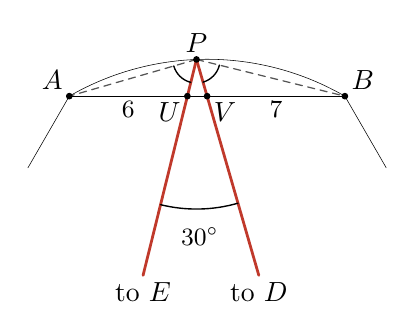
\begin{tikzpicture}
\tkzDefPoint(0.0,0.0){O} %! O = (0, 0)
\tkzDefPoint(-1.7500000,3.0310889){A} %! A = polar(O, R, 120)
\tkzDefPoint(1.7500000,3.0310889){B} %! B = polar(O, R, 60)
\tkzDefPoint(3.5000000,0.0){C} %! C = polar(O, R, 0)
\tkzDefPoint(1.7500000,-3.0310889){D} %! D = polar(O, R, 300)
\tkzDefPoint(-1.7500000,-3.0310889){E} %! E = polar(O, R, 240)
\tkzDefPoint(-3.5000000,0.000000000000000000000000000000000000000000000000015171918){F} %! F = polar(O, R, 180)
\tkzDefPoint(-0.13461538,3.4974103){P} %! P = polar(O, R, T)
\tkzDefPoint(-0.25000000,3.0310889){U} %! U = meet(P, E, A, B)
\tkzDefPoint(0.0000000000000000000000000000000000000000000000000060137206,3.0310889){V} %! V = meet(P, D, A, B)
\tkzDefPoint(-2.2750000,2.1217622){Fa} %! Fa = lerp(A, F, 0.3)
\tkzDefPoint(2.2750000,2.1217622){Cb} %! Cb = lerp(B, C, 0.3)
\tkzDefPoint(-0.81307692,0.75544062){Ee} %! Ee = lerp(P, E, 0.42)
\tkzDefPoint(0.65692308,0.75544062){Dd} %! Dd = lerp(P, D, 0.42)
%! fact on_circle(P, O, R)
%! fact dist(A, B) == 14
%! fact dist(B, C) == 14
%! fact dist(A, U) == 6
%! fact dist(V, B) == 7
%! fact dist(U, V) == 1
%! fact on_segment(U, A, B)
%! fact on_segment(V, A, B)
%! fact angle(A, P, U) == 60
%! fact angle(U, P, V) == 30
%! fact angle(V, P, B) == 60
%! fact angle(A, P, V) == 90
%! fact angle(U, P, B) == 90
%! fact equal(dist(P, A)/dist(P, B), sqrt(3)/2)
%! fact area(A, B, C, D, E, F)/sqrt(3) == 294
\tkzDrawArc(O,B)(A)
\tkzDrawSegments(A,B A,Fa B,Cb)
\tkzDrawSegments[aux](P,A P,B)
\tkzDrawSegments[key](P,Ee P,Dd)
\tkzMarkAngle[size=.3,arc=l,mark=none,mk](A,P,U)
\tkzMarkAngle[size=1.9,arc=l,mark=none,mk](U,P,V)
\tkzMarkAngle[size=.3,arc=l,mark=none,mk](V,P,B)
\tkzLabelAngle[pos=2.25,font=\small](U,P,V){$30^\circ$}
\tkzDrawPoints(A,B,P,U,V)
\tkzLabelPoint[above left,lbl](A){$A$}
\tkzLabelPoint[above right,lbl](B){$B$}
\tkzLabelPoint[above,lbl](P){$P$}
\tkzLabelPoint[below left,lbl](U){$U$}
\tkzLabelPoint[below right,lbl](V){$V$}
\tkzLabelPoint[below,lbl](Ee){to $E$}
\tkzLabelPoint[below,lbl](Dd){to $D$}
\tkzLabelSegment[below,pos=.5,len](A,U){$6$}
\tkzLabelSegment[below,pos=.5,len](V,B){$7$}
\end{tikzpicture}
\end{document}
